\section{Evaluation}
\label{sec:eval}

The evaluation asks four questions that mirror the platform's claims: whether the four concerns are genuinely replaceable without touching the core (Section~\ref{sec:eval-modularity}), whether a real eye-tracking stream drives the loop within the latency budget (Section~\ref{sec:eval-perf}), whether interventions can adapt the text while preserving the reader's context (Section~\ref{sec:eval-context}), and whether the researcher has the control and the auditable record needed to operate and reproduce experiments (Section~\ref{sec:eval-control}).
The scope is architecture and runtime feasibility, not human efficacy: with four participants, the behavioural numbers below are descriptive, and we draw no statistical inference from them.

\subsection{Setup}
\label{sec:eval-setup}

We recorded eight reading sessions on real hardware: four participants each read an expository Markdown article under two conditions, with and without the context-preserving restore (Table~\ref{tab:sessions}).
Sessions ran on a Tobii \texttt{IS4\_Large\_Peripheral} tracker under a 2560$\times$1440 display, each gated by a passing nine-point calibration validation (average accuracy 0.30 to 0.69 degrees, precision 0.08 to 0.33 degrees).
The deployment was the intended single-operator setting: backend and both surfaces on one host, traffic over the local loopback.
All eight sessions were operated in manual mode from the researcher console, and their eye-movement analysis was served live by the external provider of Section~\ref{sec:eval-modularity}.
One additional session under an advisory decision strategy exercised the decision-path instrumentation and is reported separately in Section~\ref{sec:eval-perf}.
Every number, figure, and table in this section is computed by a scripted, re-runnable pipeline from the exported session and telemetry records alone.

\begin{table}
\centering
\small
\caption{The eight recorded sessions.
Durations and counts are taken from the exported session records.}
\label{tab:sessions}
\begin{tabular}{@{}llrrrr@{}}
\toprule
 & Condition & Dur.\ (s) & Samples & Fixations & Interv. \\
\midrule
P1 & With preservation & 186 & 16664 & 656 & 5 \\
P2 & With preservation & 252 & 22688 & 1525 & 7 \\
P3 & With preservation & 171 & 15305 & 866 & 3 \\
P4 & With preservation & 224 & 20136 & 943 & 4 \\
P1 & Without & 475 & 42683 & 1914 & 9 \\
P2 & Without & 123 & 11063 & 719 & 4 \\
P3 & Without & 386 & 34624 & 1994 & 11 \\
P4 & Without & 141 & 12697 & 694 & 2 \\
\bottomrule
\end{tabular}
\end{table}

\subsection{Real-Time Feasibility}
\label{sec:eval-perf}

Across the eight sessions the tracker delivered a stable stream at its rated rate: the achieved sampling rate, computed from device timestamps, held at a mean of 89.9\,Hz (SD 0.2\,Hz), with the inter-sample interval concentrated at the nominal 11.1\,ms period.
The gaze-validity rate, the fraction of samples with at least one eye reported valid, ranged from 92.5\% to 98.0\% (mean 95.6\%) under continuous, self-paced reading rather than a constrained fixation task.

The latency budget is 100\,ms from a gaze sample to the dispatch of an intervention, the threshold below which an interface response is perceived as instantaneous \cite{miller1968response, nielsen1993responsetime} and well within the duration of a single reading fixation \cite{rayner1998eyemovements}.
The telemetry record carries the round-trip time between each client and the backend: the participant client saw a median of 1\,ms with a 95th percentile of 3\,ms, the researcher client a median of 1\,ms with a 95th percentile of 8\,ms, and no sample in either stream exceeded the budget (Figure~\ref{fig:rtt}).
These are loopback transport figures of the single-host deployment, which is the intended operating point.

The decision path is instrumented separately and is recorded only when an automated strategy is active, which the eight manual-mode sessions were not.
In the additional advisory-mode session (about 91\,s, with the reference external decision provider running out of process and every proposal gated by the researcher), the in-process decision pipeline, timed from the freshest gaze sample to proposal dispatch, had a median latency of 6\,ms, a 95th percentile of 11\,ms, and a maximum of 46\,ms across 14015 samples, while the round trip to the provider had a median of 5\,ms and a maximum of 7\,ms across its eight proposals.
Both legs stayed within budget, but we read this as a validation of the instrumentation under a rule-based reference provider on one host, not as a campaign-scale result.

\begin{figure}
  \centering
  
\includegraphics[width=0.94\columnwidth]{figures/eval-client-rtt.pdf}
  \caption{Cumulative distribution of client round-trip time for the participant and researcher clients against the 100\,ms budget.
  Every sample falls within budget.}
  \Description{A cumulative distribution plot with two curves rising steeply near one millisecond and reaching one hundred percent far to the left of a dashed vertical line marking the one hundred millisecond budget.}
  \label{fig:rtt}
\end{figure}

\subsection{Modularity and External Providers}
\label{sec:eval-modularity}

The dependency rule that makes the modules replaceable is enforced twice: the build itself admits no reference from the core outward, and an executable boundary test inspects the loaded assemblies and fails if the domain or application core depends on infrastructure, transport, or host code.
Adding an in-process intervention module requires one registration entry and edits to no existing module, because the runtime resolves modules from registries by identifier.

The stronger test is out of process.
Three external providers connect to the running platform over the documented provider protocol: a reference decision provider and a reference analysis provider written by us, and a connector that bridges the reading-difficulty pipeline of a concurrent, independent master's project at our institution to the analysis seam.\footnote{\emph{Reading the Struggle}, by Katarina Kraljevi\'{c} and Sree Keerthi Desu (DTU).
Their pipeline derives reader-struggle signals (cognitive load, reading style, and a pupillary load index) from eye-tracking features; our connector adapts it to the analysis contract and uses their code unmodified.
\todopaper{Check whether their thesis is now submitted and citable, and cite it here if so.}}
The reference providers, written by the contract's own authors, evidence only that the contract is sufficient; the third goes further, because we neither wrote its pipeline nor designed the contract around it, its addition changed nothing in the backend, and, most tellingly, it served as the live analysis source for the eight evaluation sessions themselves.
The fixation, saccade, and regression events reported throughout this section were produced by that independent team's code running behind the platform's contract.

\subsection{Context Preservation}
\label{sec:eval-context}

The eight sessions form a with-and-without comparison of the context-preserving restore.
In the enabled condition the restore ran together with its highlight cue, so the conditions contrast a bundle (positional restore plus a brief highlight of the resume point) against neither; we return to this confound below.
Because preservation acts in the moments after a reflow, both behavioural measures are aligned to each intervention rather than averaged over sessions, which leaves the conditions with unequal counts: 19 interventions with preservation and 26 without.

Reading-resume time, the interval from an intervention to the reader's next forward saccade, was shorter with preservation (median 482\,ms, mean 670\,ms) than without (median 650\,ms, mean 923\,ms), as shown in Figure~\ref{fig:rrt}.
The regression rate in the five seconds after an intervention showed the same separation: 23\% with preservation, down from a 29\% pre-intervention baseline, against 33\% without, essentially unchanged from its 32\% baseline (Figure~\ref{fig:postreg}).
The pattern held across three-, five-, and ten-second windows, and the resume-time direction held for three of the four participants.
We state the direction of these numbers without inferring from them: four participants and an unevenly split sample do not support inference, and the bundled highlight means the difference cannot be attributed to the restore geometry alone, the more so as prior work found highlighting to be the component driving recovery improvement \cite{jensen2025context}.

\begin{figure}
  \centering
  
\includegraphics[width=0.85\columnwidth]{figures/eval-rrt.pdf}
  \caption{Reading-resume time per intervention by condition (19 interventions with preservation, 26 without; bars mark medians).
  Descriptive only.}
  \Description{A dot plot with two columns of points, one per condition. The with-preservation points sit lower, with median bars at 482 and 650 milliseconds.}
  \label{fig:rrt}
\end{figure}

\begin{figure}
  \centering
  
\includegraphics[width=0.85\columnwidth]{figures/eval-post-regression.pdf}
  \caption{Regression rate in the five seconds before and after each intervention, by condition.
  Without preservation the rate rises after the intervention; with preservation it falls below its baseline.
  Descriptive only.}
  \Description{A paired plot of regression rates before and after interventions for the two conditions, showing a decrease with preservation and a slight increase without.}
  \label{fig:postreg}
\end{figure}

\paragraph{Self-measurement catches a defect.}
Within the four preservation-enabled sessions, the reader recorded a graded outcome for every intervention: the displacement the reflow induced and the residual after the restore.
Sixteen of the nineteen outcomes were graded degraded, and for those the median residual was 389\,px against a median induced displacement of only 38\,px.
The restore was moving readers substantially further than the reflow it compensated.
The cause was the original strategy's fixed target: it re-established the committed sentence near the top of the reading area regardless of how far the reader actually sat from it, so the smaller the reflow, the worse the compensation.

\paragraph{A deterministic sweep, and the revision.}
The live outcomes are observational, covering whatever interventions the participants happened to receive.
To measure displacement under controlled conditions, a measurement harness mounts the real participant reader outside a live session and drives the same restore hook over every built-in layout intervention from six reading positions, with preservation off and on: 66 trials per condition.
Table~\ref{tab:displacement} reports the median on-screen displacement of the word the reader was on (one reading line is 32.4\,px).
Without preservation the median displacement is 34.3\,px, though heavy-tailed (a six-point font enlargement moves the word 142\,px, and line-width changes, which repaginate, up to 188\,px).
With the original restore, preservation made displacement worse rather than better: the median tripled to 104.4\,px, the restore moved the word further than the bare reflow in 45 of 66 trials, and the effect was starkest for the smallest changes (a letter-spacing step that moves the word not at all was thrown 115\,px).
The revised restore returns the captured reading position to the viewport offset it held before the change (Section~\ref{sec:platform-context}).
It removes the over-repositioning (4 of 66 trials) and brings the median displacement to 32.4\,px, at or below the no-preservation baseline, with the gains concentrated exactly where reflows are large; line-width changes repaginate and lie beyond what a within-page restore can compensate.
Figure~\ref{fig:overreposition} shows both restore versions against the line of equality.
The revision is verified geometrically by this sweep; its behavioural benefit to readers has not yet been re-measured.

\begin{table}
\centering
\small
\caption{Median on-screen displacement (px) of the word being read, per intervention, from the 66-trial deterministic sweep: without preservation, with the original (top-of-area) restore, and with the revised (offset-preserving) restore.
Lower is better; one reading line is 32.4\,px.}
\label{tab:displacement}
\begin{tabular}{@{}lrrrr@{}}
\toprule
Intervention & n & Without & Original & Revised \\
\midrule
Font size $+2$\,px & 6 & 24.5 & 168.3 & 24.5 \\
Font size $+6$\,px & 6 & 142.4 & 225.2 & 43.0 \\
Font size $-2$\,px & 6 & 38.0 & 82.7 & 54.0 \\
Line height $+0.3$ & 6 & 35.4 & 124.7 & 35.4 \\
Line height $-0.3$ & 6 & 34.5 & 53.7 & 31.7 \\
Line width $-120$\,px & 6 & 188.2 & 156.2 & 188.2 \\
Line width $+80$\,px & 6 & 161.9 & 148.6 & 148.6 \\
Letter spacing $+0.06$\,em & 6 & 0.0 & 115.0 & 0.0 \\
Letter spacing $+0.12$\,em & 6 & 32.4 & 154.8 & 16.3 \\
Font family $\to$ Inter & 6 & 1.0 & 31.3 & 1.0 \\
Font family $\to$ Space Grotesk & 6 & 0.0 & 49.5 & 0.0 \\
\midrule
\textbf{Overall} & 66 & \textbf{34.3} & \textbf{104.4} & \textbf{32.4} \\
\bottomrule
\end{tabular}
\end{table}

\begin{figure}
  \centering
  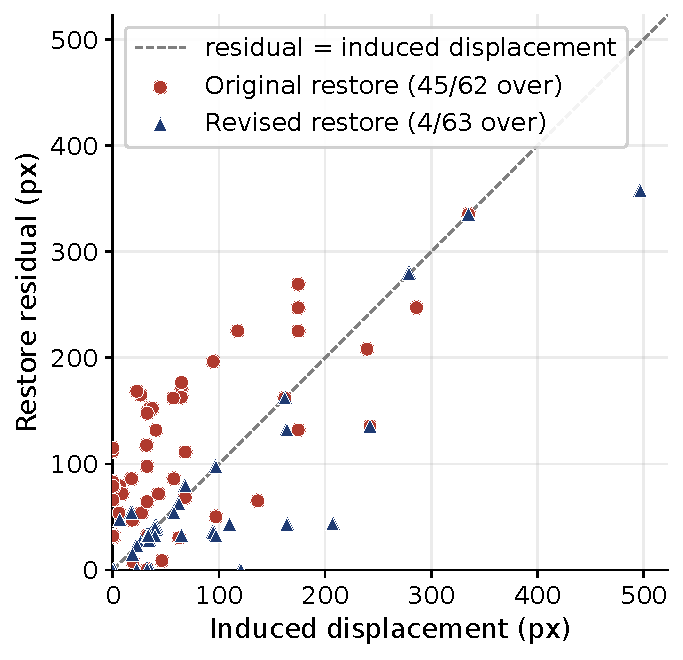
\includegraphics[width=0.9\columnwidth]{figures/eval-restore-overreposition-fixed.pdf}
  \caption{Restore residual against the displacement the reflow induced, one point per sweep trial for which the reading word stayed on screen in both conditions.
  The original restore (circles) lies above the line of equality for most trials (45 over-repositions); the revised restore (triangles) returns onto or below it (4).}
  \Description{A scatter plot of residual versus induced displacement with a dashed diagonal line of equality. Circle markers cluster above the diagonal; triangle markers lie on or below it.}
  \label{fig:overreposition}
\end{figure}

\subsection{Researcher Control and Reproducibility}
\label{sec:eval-control}

All recorded sessions were operated end to end through the gated researcher console: no session started before its readiness gates and calibration validation passed, every intervention in Table~\ref{tab:sessions} was applied from the console during the run, and the participant's view was mirrored throughout.
Reproducibility is demonstrated by construction: every figure and table in this section was produced from the exported session and telemetry records alone, with no reference to live state, and the replay view reconstructs any recorded session from its export.
